%%%%%%%%%%%%%%%%%%%%%%%%%%%%%%%%%%%%%%%%%%%%%%%%%%%%%%%%%%%%%%%%%%%%%%%%%%%%%%%%
%2345678901234567890123456789012345678901234567890123456789012345678901234567890
%        1         2         3         4         5         6         7         8

\documentclass[letterpaper, 10 pt, conference]{ieeeconf}  % Comment this line out if you need a4paper


%\documentclass[a4paper, 10pt, conference]{ieeeconf}      % Use this line for a4 paper

\IEEEoverridecommandlockouts                              % This command is only needed if 
% you want to use the \thanks command

\overrideIEEEmargins

% Sorts and compresses references properly
% (poor substitute for natbib, but it's the best we can do with this docclass)
\usepackage{cite}

% Give us pretty subfigures
\usepackage{subfig}

% Good math support
\usepackage{mathtools}
\usepackage{amssymb}
\usepackage{graphicx}
\usepackage{caption}
\DeclareCaptionFont{eightpt}{\fontsize{8pt}{9pt}\selectfont #1}
\captionsetup{font=eightpt}

\graphicspath{{figures/}}

% Needed to meet printer requirements.

% See the \addtolength command later in the file to balance the column lengths
% on the last page of the document

% The following packages can be found on http:\\www.ctan.org
%\usepackage{graphics} % for pdf, bitmapped graphics files
%\usepackage{epsfig} % for postscript graphics files
%\usepackage{mathptmx} % assumes new font selection scheme installed
%\usepackage{times} % assumes new font selection scheme installed
%\usepackage{amsmath} % assumes amsmath package installed
%\usepackage{amssymb}  % assumes amsmath package installed


\title{\LARGE \bf
	I Picture You: \\
	Imaginative localization on remote teammates
}
% Automated synthesis of scalable algorithms for inferring non-local
%properties to assist in multi-robot teaming


\author{Taeyeong Choi, Sehyeok Kang, and Theodore P.~Pavlic % <-this % stops a space
	\thanks{*This work was not supported by any organization}% <-this % stops a space
	\thanks{T.~Choi, S.~Kang, and T. P.~Pavlic are with the School of Computing, Informatics, and Decision Systems Engineering,
		Arizona State University, Tempe, AZ 85281, USA
		{\tt\small \{tchoi4, skang66, tpavlic\}@asu.edu}}%
}


\begin{document}
	
	
	
	\maketitle
	\thispagestyle{empty}
	\pagestyle{empty}
	
	
	%%%%%%%%%%%%%%%%%%%%%%%%%%%%%%%%%%%%%%%%%%%%%%%%%%%%%%%%%%%%%%%%%%%%%%%%%%%%%%%%
	\begin{abstract}
		
		We propose \emph{IPY-Net}, as an extension of \cite{Choi17}, to tackle the Remote Teammate 
		Localization (RTL) problem where a robot embedded in a multi-robot team is to predict positions 
		of all other teammates when each robot has a limited sensor radius and a 
		relatively simple motion rule with dependency on the position of its nearest neighbors. 
		The previous work presented feasibility of a scalable machine learning approach for the 
		predicting robot to proactively assist a team behavior in caging scenario. 
		In this work, \emph{IPY-Net} is designed to improve scalability by taking into account
		physical constraints on the team formation as well as producing probabilistic predictions  
		in the form of image through deep learning pipeline.
		Furthermore, while we previously relied only on computer simulations, 
		all experiments in this work are performed in a physical robotic platform, \emph{Thymio}, 
		to demonstrate the performance gain in more realistic environments. 
		
	\end{abstract}
	
	
	%%%%%%%%%%%%%%%%%%%%%%%%%%%%%%%%%%%%%%%%%%%%%%%%%%%%%%%%%%%%%%%%%%%%%%%%%%%%%%%%
	
	\section{Introduction}
	\label{sec:intro}
	
	In multi-robot systems including swarms, every robot is usually allowed to observe 
	only a subset of its team members and interact with them to determine the next action 
	according to relatively simple motion rules. 
	Such a property enables the entire system to perform in a distributed manner, and 
	also the behavior of it can be driven easily by a few leader robots to 
	eventually achieve the goal [x]. 
	This implies that if a robot has an ability to recognize useful property, e.g.) formation, 
	of the whole team in real time using its local sensors, 
	it could present adjustive actions accordingly to better promote a collective behavior 
	for the sake of the team.
	
	In \cite{Choi17}, we suggested a machine learning method to solve the 
	RTL problem where a robot embedded in a multi-robot team is to predict 
	positions of all other teammates using only local observations about a single nearby teammate. 
	Since each robot has a limited sensor radius and a relatively simple motion rule with dependency 
	on the position of its nearest neighbors in line formation, 
	the predicting robot has to be able to learn the regularity 
	of the observed motions. Through simulated experiments, we showed the feasibility of the idea 
	especially in caging scenario in which the predicting robot could recognize the team behavior and 
	use a proactive maneuver accordingly. 
	
	RTL problem provides some unique characteristics compared to general localization problems. 
	In RTL, the robot that executes predictions does not try to localize itself but its teammates using 
	accessible observations. 
	Moreover, the robot is not allowed to communicate with other members during prediction phase to 
	consider communication-free scenarios, which differs from works on cooperative localization. 
	Hence, RTL usually assumes that robots behave with correlations with their neighbors so that 
	the resulting behaviors contain the state information of their neighbors. 	
	In this sense, state observers in networked robotic system could be a more similar 
	configuration to RTL, but RTL emphasizes 
	possible applications to variable sizes of robotic system and also a general framework 
	that would not impose any constraint on dynamics of the system.
	
	%
	\begin{figure}\centering
		\includegraphics[width=1.\columnwidth]{fig_Concept}
		\caption{Example of \emph{IPY-Net} performing RTL on $6$-robot team. 
			While the \emph{Head} (red) is driving 
			the team in line formation, the \emph{Tail} can observe the motions of 
			\emph{Follower 1} (purple) within its sensor radius (yellow).
			The observation, $O$, and the historical positions of all robots, $h$, that
			the \emph{Tail} has known so far become an input to \emph{IPY-Net} to pro 
			All positions of robots in the local view of \emph{Tail} are visualized in 
			image as probabilistic representation. Note here that since \emph{Follower 4} 
			can be observed directly, the image representation does not illustrate any
			uncertainty for it. 
		}
		\label{fig:Concept}
	\end{figure}
	%
	
	In this work, we propose \emph{IPY-Net} to significantly reduce prediction errors solving 
	the RTL problem, which would allow to gain stable performance even with more robots added. 
	\emph{IPY-Net} runs a deep neural network as a backbone, 
	first to consider physical constraints on the sequential change of team formation and, 
	second to use a probabilistic representation in the form of image for obtained observations and 
	new predictions. Specifically, every observed or predicted position is 
	encoded as an image in which the summation of all values must be $1$, which can be
	viewed as a probability distribution of position of the robot. Hence,
	\emph{IPY-Net} learns how to synthesize inputs with some uncertainty to produce a probabilistic 
	prediction outcome in end-to-end fashion. Furthermore, a recurrent layer is deployed in \emph{IPY-Net}, 
	which enables the model to take into account possible evolution of 
	team formation based on recent history and reduce the searching space for predicted solution. 
	With all combined, historical probabilistic (soft) formations are used as input per prediction
	providing more flexibility to the predictor in selecting salient features and finally leading to 
	more robust performance even when the input is noisy to some level.
	
	We conduct all experiments on a physical robotic platform,
	\emph{Thymio} \cite{Shin14}, to demonstrate the improvement in more realistic environments in 
	contrast to the previous work that relied only on computer simulations. 
	All codes are available online\footnote{http://www.github.com/ctyeong}, and supplementary videos 
	are submitted as well. 
		
	This paper is organized as follow. 
	In Section~\ref{sec:related_work}, we explore related literature and the distinction of our work. 
	Section~\ref{sec:problem_description} explains more details about our setting of RTL problem. 
	Then, we introduce our method, \emph{IPY-Net}, in Section~\ref{sec:method}, and 
	Section~\ref{sec:experiments} explains details about experiments performed on real robots, 
	including data collection, hyperparameters used for learning, and the results. 
	Lastly, we summarize our research and discuss future directions 
	in Section~\ref{sec:discussion_and_future_work}.
	
	\section{Related work}
	\label{sec:related_work}
	
		%
	\begin{figure*}\centering
		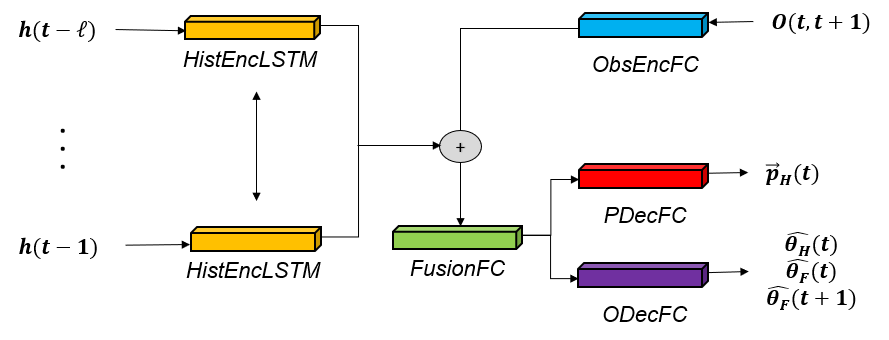
\includegraphics[width=1.8\columnwidth]{fig_DL_Pipeline}
		\caption{Structure of \emph{IPY-Net}. This is an snapshot example when applied to a focused module of
			$3$~robots, called \emph{Tail, Follower, Head} within it, at time $t$. 
			The Encoder-Decoder structure encodes
			1) historical positions and orientations of \emph{Follower} and \emph{Head} 
			until $t-2$ and 2) the observed positions of the \emph{Follower} at $t-1$ and $t$. 
			The decoder part learns to estimate 1) the position of \emph{Head} at $t-1$ and 
			2) orientations of \emph{Follower} at $t-1$ and $t$ and \emph{Head} at $t-1$.   
		}
		\label{fig:DL_Pipeline}
	\end{figure*}
	%
	
	\section{Problem Description} 
	\label{sec:problem_description}
	
	\section{Method}
	\label{sec:method}
	
	
	\section{Experiments} 
	\label{sec:experiments} 
	
	
	\begin{table}[]
		\label{table:data_description}
		\begin{tabular}{|c|c|c|c|c|}
			\hline
						&  Duration & Num. of Samples & Num. of Instances  \\ \hline
			$3$ robots & $120$ minutes & $2,000$ & $500$  \\ \hline
			$5$ robots & $60$ minutes  & $1,000$ & $250$  \\ \hline
		\end{tabular}
		\caption{Description of data collected from executions of $3$-robot and $5$-robot teams.}
	\end{table}
	
	
	To demonstrate the effectiveness of our method, we employ a physical robotic platform, 
	\emph{Thymio} \cite{Shin14}, which allows to execute a team of small two-wheeled mobile robots.   
	We use a central computer connected with a overhead camera to simulate better proximity 
	sensors, a more powerful computing power, and a GPS system that would easily run on each robot in 
	real scenarios. The central system is set up to detect the locations of robots in real time 
	and communicate with a \emph{Raspberry Pi} board \cite{Upton14} on each robot to send
	the next command relying on its neighbors. Although the experiment configuration involves 
	such external computations and sensors due to limited capability of \emph{Thymio}, 
	most of realistic assumptions hold, and the robots are still influenced by 
	physical constraints and disturbance in motion. For better understanding of readers, 
	we submit a supplementary video. 
	
	The location detection is performed at $4$ frames per second at each of which 
	a new command is received by each robot. Also, 
	all coordinates and orientations at $2$ frames per second are collected, which 
	is not necessarily synchronized with the command timing. 
	
	Two different sizes of robot team are deployed throughout following experiments: 
	$3$~robots and $5$~robots in which the \emph{Head} robot continues to receive a command to 
	move to an arbitrary destination point nearby in a $OO \times OO$ meters arena. 
	Table~\ref{table:data_description} shows details about the data collected from 
	each configuration where a sample refers to a set of coordinates and orientations recorded 
	at an instant time step, and an instance is a sequence of samples for $13$ seconds. 
	The instances are clustered to have at least $7$-second time gap to another so that
	the motions between separate ones have only little dependency. 
	
	$70$\% data from the $3$-robot team is used to train \emph{IPY-Net} by feeding each sample, 
	and the rest $20$\% is used for test. 
	The trained model is also tested with the $5$-robot team, in which the relay prediction is 
	initialized at the beginning of each instance. 
	The length of history is set to $5$~seconds to accept inputs for past $10$~time steps, and 
	the predictions occur for the next $8$~seconds.  
	 	
	\emph{IPY-Net} is implemented in \emph{Tensorflow} \emph{Python} library \footnote{https://www.tensorflow.org/} 
	to realize the entire pipeline. The evaluation is reported in Euclidean distance between 
	the predicted position and the truth, using the model that achieves the best performance 
	during $100$ epochs, by which the loss mostly converges to zero. 

	We compare our proposed model to four different approaches such as: 
	\begin{itemize}
		\item \emph{$2$X Heuristic}: 
		The prediction on \emph{Head} within a modular team is performed by doubling the vector 
		$\vec{p}_{F} - \vec{p}_{T}$.
		
		\item \emph{FC}: 
		Two fully connected layers run in the predictor without considering historical 
		information, which is based on \cite{Choi17}.  
				
		\item \emph{LSTM-FC}: 
		Model combining the historical LSTM and FC layers similar to \emph{IPY-Net} except that 
		all inputs and outputs are represented as numerical values instead of images. 
		
		\item \emph{I-LSTM-FC}: 
		Imaginative model using the same structure as \emph{IPY-Net} with difference that 
		only best predictions on coordinates or orientation are preserved from each predicted image. 
		As needed, the preserved information is processed to generate a new image input during 
		relay prediction process.
	\end{itemize}	

%	\subsection{Data collection} 
%	\label{sec:data_collection}
	
	
%	\subsection{Results} 
%	\label{sec:results}
	
	\subsection{Overall accuracy}
	\label{sec:overall_performance}
	
	
	\subsection{Microscopic analysis}
	\label{sec:microscopic_analysis}
	
	Here, we highlight the behavior of 
	
	
	\subsection{Qualitative results} 
	\label{sec:qualitative_results} 

%	Specifically, the position information is projected onto a two
%	dimensional vector as an image, while orientation is on a one dimensional vector.
%	Since each vector basically represents a probability distribution, where the sum of all values 
%	must be $1$, the representation of obtained observation has $1$ for the corresponding element
%	and $0$ for others. Therefore, \emph{IPY} is trained to produce a probability distribution of 
%	predicted positions and orientations of its teammates. 
	
%	\emph{IPY} also takes into account the historical state information known so far, 
%	since it can regulate the predictor on current observation of neighbor as well as
%	physical constraints on the global formation. To deal with the historical imaginative 
%	representation, \emph{IPY} performs with a stack of convolutional layers and a recurrent
%	layer. 
		
%	We use a physical robotic platform, \emph{Thymio}, to demonstrate the effectiveness of 
%	our proposed methods, although \cite{Choi17} relied only on computer simulations.
%	We compare performances of a model in \cite{Choi17}, general state-of-the-art models, 
%	and some variants of \emph{IPY} to show how errors increase as more robots are employed in 
%	general and how \emph{IPY} alleviates it by the imaginative representation. 

	\section{Discussion \& Future work}
	\label{sec:discussion_and_future_work}
	
	We have shown \emph{IPY-Net}, a powerful approach to tackle the remote localization problem 
	where a robot with limited sensors is to predict positions of all others only using 
	observations about its nearest neighbor. 
	\emph{IPY-Net} follow the fundamental spirit of \cite{Choi17} to apply a predictor 
	trained for a small robot team to a chain of them in a larger team, since it 
	can provide a scalable feature without re-training.   
	The distinction in \emph{IPY-Net} is , however, to use a sequence of historical knowledge and 
	make predictions based on imagination of robot states including position and orientation.
	We expected learning with history would help regulate the model on physical constraints on 
	the team formation, and also the imaginative representation could contain 
	certainty about the prediction, which would bring about more robust performance. 
	
	The experiment results were obtained using a realistic robotic platform to prove 
	that our method outperforms not only the regressor
	introduced in \cite{Choi17} but also a general state-of-the-art neural network 
	model that is able to use historical data. Especially, our model can present 
	stable performance even when the input contains some errors which have occurred in 
	previous prediction. 
	  
	
	In future work, 
	
	
{\small
	\bibliographystyle{IEEEtran}
	\bibliography{IEEEabrv, IEEEexample}
}


\end{document}
